\chapter{Travaux associés}
\label{travail associé}
Cette partie donne un aperçu de l'existant en matière d'apprentissage de la programmation.

Premièrement, il y aura un tour d'horizon des politiques gouvernementales de pays qui ont adopté l'apprentissage de la programmation dans leur programme officiel. Ceci présentera les avancées de cette problématique et aidera à envisager différentes manières de la traiter. 

Après ce tour d'horizon, l'attention sera portée sur des organisations non gouvernementales qui ont pour but de promouvoir l'enseignement de la programmation. 

La troisième partie décrira les langages utilisés dans les organisations présentées précédemment. 

Enfin, des concepts différenciateurs seront extraits de chaque initiative afin les distinguer l'une de l'autre.
\section{État de la programmation dans le monde}
\label{monde} %TODO dire pourquoi la politique influe sur la problématique
Cette section fait un tour d'horizon de différents pays qui enseignent la programmation aux jeunes. L'accent est mis spécialement sur leur positionnement politique et leur manière d'intégrer l'apprentissage de la programmation.
\subsection{Angleterre}
L'apprentissage de l'informatique en Angleterre\footnote{\url{https://www.gov.uk/government/collections/statutory-guidance-schools\#national-curriculum-from-september-2014}} n'est pas nouveau. Pendant longtemps, il était centré sur les technologies de l'information et de la communication (TIC). C'est donc principalement l'utilisation de l'informatique, et non sa conception qui était enseignée.

En 2010, une étude a été commandée à la Royal Society pour évaluer cet apprentissage. Un an plus tard, le rapport a révélé que l'enseignement n'est ni efficace ni en adéquation avec l'évolution de l'informatique dans leur société. La Royal Society suggère d'adapter les matières abordées en informatique en enseignant l'apprentissage de la programmation. Sur base de ce rapport, les programmes de cours ont été modifiés en 2012.

\subsection{France}
En France\footnote{\url{http://fr.wikipedia.org/wiki/Informatique\_et\_sciences\_du\_num\%C3\%A9rique}
\url{http://fr.wikipedia.org/wiki/Baccalaur\%C3\%A9at\_scientifique}}, depuis deux ans, l'informatique fait partie intégrante du programme du baccalauréat de type S. Une des matières dispensées est "Informatique et sciences du numérique". Cette matière se subdivise en quatre sous parties : représentation de l'information, algorithmique, langage et programmation, architectures matérielles. Cette approche est donc également basée sur l'apprentissage de la programmation plutôt que sur les TIC.

\subsection{Corée du Sud}
La Corée du Sud enseigne l'informatique depuis longtemps et à tous les niveaux de l'enseignement. La culture numérique dans les pays asiatiques est fort différente de ce que l'on connait chez nous. Par exemple, une carrière dans le jeu vidéo est quelque chose de tout à fait normal. L'informatique est vraiment omniprésente dans cette culture, il est donc normal que son apprentissage commence dès l'enseignement fondamental.

\subsection{Grèce}
L'apprentissage des sciences informatiques prend une place importante dans les programmes grecs. Dès 6 ans, les enfants sont confrontés à l'informatique à l'école. À cet âge, ils apprennent principalement la maîtrise de l'outil. Dès 10 ans, leurs cours d'informatique prennent une tournure plus algorithmique et donc plus proche de la science de l'informatique.

\subsection{Nouvelle-Zélande}
Ce pays a adopté récemment les sciences informatiques dans son programme d'étude. Les cours sont dispensés à partir de 15 ans. Ces cours comprennent l'apprentissage de la programmation et de concepts informatiques en général. La nouvelle-Zélande, en introduisant les cours tardivement, s'inscrit dans une logique similaire à la France sans toute fois restreindre l'informatique aux options scientifiques.

\subsection{La belgique \ldots}
%TODO to be 
L'apprentissage de la programmation est déjà bien avancé dans plusieurs pays. Ce n'est malheureusement pas encore tout à fait le cas dans le nôtre. En effet, quelques initiatives locales existent, mais aucune décision politique n'a été prise jusqu'à présent.\\
\section{Organisations existantes}
Il sera présenté ici un ensemble d'initiatives à ce travail qui s'inscrivent la logique de ce travail. Elles sont toutes non gouvernementales et proposent d'enseigner la programmation de différentes manières.
\subsection{Code.org}
\begin{figure}[!ht]
  \begin{center}
    
\includegraphics[scale=0.5]{content/5-related_work/images/code}
    \caption{Logo de code.org}
    \label{fig:code.org}
  \end{center}
\end{figure}
Code.org \cite{code-org-about} est une organisation sans but lucratif des USA qui a pour objectifs :
\begin{itemize}
  \item apporter l'informatique dans toutes les classes de \gls{secondaire} aux États-Unis ;
  \item démontrer le succès de l'utilisation de cours en ligne dans l'enseignement public ;
  \item ajouter l'informatique dans les bases des programmes de sciences et de mathématique des 50 états ;
  \item employer la connaissance technique collective pour améliorer l'apprentissage de l'informatique dans le monde ;
  \item augmenter la représentation féminine et de personnes de couleurs dans l'informatique.
\end{itemize}

Pour ce faire, Code.org fournit une plate-forme \cite{code-org-20hr} web qui permet aux professeurs de suivre leurs élèves grâce à un système de classes. Ce programme d'apprentissage se base sur Blockly (voir \ref{blockly}).

Toutes les ressources sont gratuites et librement utilisables \cite{code-org-faq}. Elles sont conçues pour que les professeurs comme les élèves puissent commencer le cours sans connaître l'informatique (une assistance gratuite est proposée au professeur si nécessaire).

Le site propose aux professeurs de se faire récompenser s'ils arrivent à finir les 27 \glspl{mission} proposées avec minimum 15 élèves. Dans ce cas, ils gagnent $750\$$. S'ils ont au moins 7 filles dans le groupe, ils peuvent prétendre à $250\$$ supplémentaires.

\subsubsection{Déroulement des leçons}
Code.org propose des sessions d'une heure de travail/jeu/apprentissage. Chaque unité est découpée en \glspl{mission} courtes (ex:5-20) apportant un concept de programmation. Avant chaque concept, une petite vidéo l'introduit et donne des exemples d'utilisation.

Il propose de faire travailler les élèves en binôme \cite{wiki-pair-prog}, ce qui entraîne moins de questions au professeur et permet de mieux s'approprier la matière. Le travail par binôme casse également l'image du "geek" et montre que la programmation est une science sociale et collaborative. De plus, moins d'ordinateurs sont nécessaires.

Le site explique également que pour faire participer tous les élèves, il faut avoir confiance en leurs compétences. La philosophie est d'inciter les premiers groupes à aider les derniers.

Quand un élève a une question, Code.org recommande de la soumettre à 3 de ses camarades avant de la poser au professeur. Cela permet aussi d'éviter les questions de distraction ou de manque de compréhension.

Pour chaque petite \gls{mission}, un test automatisé informe si la \gls{mission} est réussie ou non. Si celle-ci est réussie, la plateforme propose la \gls{mission} suivante. Dans les premières \glspl{mission}, il y a également un compteur de \glspl{bloc} qui informe du nombre de \glspl{bloc} nécessaires pour réaliser la \gls{mission} de manière optimale.

\subsection{CoderDojo}
\begin{figure}[!ht]
  \begin{center}
    
\includegraphics[scale=0.5]{content/5-related_work/images/dojo}
    \caption{Logo de CoderDojo}
    \label{fig:coder dojo}
  \end{center}
\end{figure}
CoderDojo \cite{dojo-about} est un réseau open source de Clubs de programmation dans le sens le plus large du terme. Tous les dojos sont donc autonomes. Des enfants de 5 à 17 ans y apprennent la programmation (site web, application, jeux...). La seul règle est "Above All : Be Cool" qui est mise en pratique en créant simplement des espaces d'échanges de savoirs amicaux et sociables.

CoderDojo a été créé par James Whelton, un irlandais de 18 ans, et Bill Liao, un entrepreneur australien à Cork. James, après avoir hacké l'iPod nano, a eu des demandes de jeunes enfants pour avoir des cours de programmation. Beaucoup de gens de Dublin ont été à ses cours et donc un nouveau Dojo y a été créé. Ensuite, cela s'est étendu à tout le globe.

\subsection{Code Club}
\begin{figure}[H]
  \begin{center}
    
\includegraphics[scale=0.3]{content/5-related_work/images/club}
    \caption{Logo de Code Club}
    \label{fig:code club}
  \end{center}
\end{figure}
Code Club\cite{codeclub-about} est un réseau national de Clubs mené par des bénévoles en dehors des heures de cours. Leurs activités s'adressent à des enfants de 9 à 11 ans.

Ils créent le matériel pour permettre à des bénévoles de donner des cours parascolaires d'environ une heure par semaine. Ils proposent d'utiliser dans cet ordre scratch, HTML/css et puis Python. Ils ont pour objectif que les 21000 écoles \glspl{fondamental} anglaises aient leur club.

Leur philosophie est de favoriser l'amusement, la créativité et l'exploration avant l'apprentissage des concepts de programmation.

\subsection{KidsCode}
\label{init-kidscode}
\begin{figure}[!ht]
  \begin{center}
    
\includegraphics[scale=0.5]{content/5-related_work/images/kidscode}
    \caption{Logo de KidsCode}
    \label{fig:kidscode}
  \end{center}
\end{figure}
KidsCode \cite{kidscode} est une petite initiative wallonne qui organise actuellement un stage pour les enfants de 10 à 14 ans. Les ateliers sont dispensés par deux informaticiens qui proposent de partager leur passion. Ils encadrent les jeunes de manière ludique dans le but de les rendre autonomes.

KidsCode propose d'apprendre la programmation grâce au langage Python. Ce langage a été choisi pour sa facilité tout comme pour son utilisation en condition réelle.

KidsCode a été conçu et pensé en association avec l'incubateur de startup Nestup. Cette initiative est le fruit du constat par les entreprises, d'un manque d'intérêt pour la programmation chez les plus jeunes. Ceci entraîne un manque de vocations dans les startups.

\section{Langages de programmation}
\label{langages}
Cette partie traite des différents éditeurs et langages de programmation utilisés dans les organisations présentées au point précédent.

\subsection{Blockly}
\label{blockly}

\begin{figure}[!ht]
  \begin{center}
    
\includegraphics[scale=0.5]{content/5-related_work/images/blocky}
    \caption{Logo de Blocky}
    \label{fig:blocky}
  \end{center}
\end{figure}
Blockly \cite{blockly} est un langage de programmation graphique basé sur des technologies du web.

Blockly a comme particularité :
\begin{itemize}
\item de s'exécuter dans un navigateur ;
\item d'exporter du code source en JavaScript, Dart, etc. ;
\item d'être open source ;
\item d'être haut niveau.
\end{itemize}

Il n'est pas directement une plateforme d'éducation dans le sens où, il peut être utilisé autant pour l'éducation, le business, des jeux, \ldots en fonction des \glspl{bloc} implémentés.\\

Blockly a été conçu avec certaines propriétés choisie lors de sa création. Les trois premières augmentent la compréhension des néophytes, les autres portent sur des facilités du langage. Les propriétés décidées lors de la conception du langage sont \cite{blockly-lang} :

\begin{itemize}
  \item des indices de listes commençant à 1 ;
  \item des noms de variables non sensibles à la casse ;
  \item pas de portée de variable, elles sont toutes globales ;
  \item la possibilité de faire un export en JavaScript ;
  \item un code natif généré proche de celui des \glspl{bloc}.
\end{itemize}

\subsection{Scratch}

\begin{figure}[!ht]
  \begin{center}
    
\includegraphics[scale=0.4]{content/5-related_work/images/scratch}
    \caption{Logo de Scratch}
    \label{fig:scratch}
  \end{center}
\end{figure}
Scratch \cite{scratch} est un langage de programmation graphique développé par le MIT pour apprendre aux enfants la programmation. C'est l'interface qui permet de faire des scripts facilement grâce à une programmation par \glspl{bloc} et du glisser-déposer.\\

Il a été pensé pour être un outil créatif pour réaliser des histoires, des jeux, des simulations, de l'art, etc. Il a, par exemple, son propre éditeur d'image et de sons. Un autre but de ce langage est d'être simple à utiliser et à apprendre. Il a en effet été conçu pour des enfants n'ayant aucune connaissance préalable en programmation.\\

Actuellement Scratch est à sa version 2 qui est une version web. Cette version a été complètement réécrite en flash par rapport à la version 1 en Smalltalk. De plus, la version 2 n'est plus open source contrairement à la première version.

Comme le montre la figure \ref{fig:scratch-printscreen}, l'interface de Scratch se divise en plusieurs grandes parties :

\begin{enumerate}
\item sur la gauche, il y a la zone de dessin dans laquelle s'anime les composants graphiques des scripts ;
\item au milieu, une liste des \glspl{bloc} disponible triés par catégorie ;
\item sur la droite, la zone de script qui contient tous les scripts liés au sprite sélectionné.
\end{enumerate}

\begin{figure}
  \begin{center}
    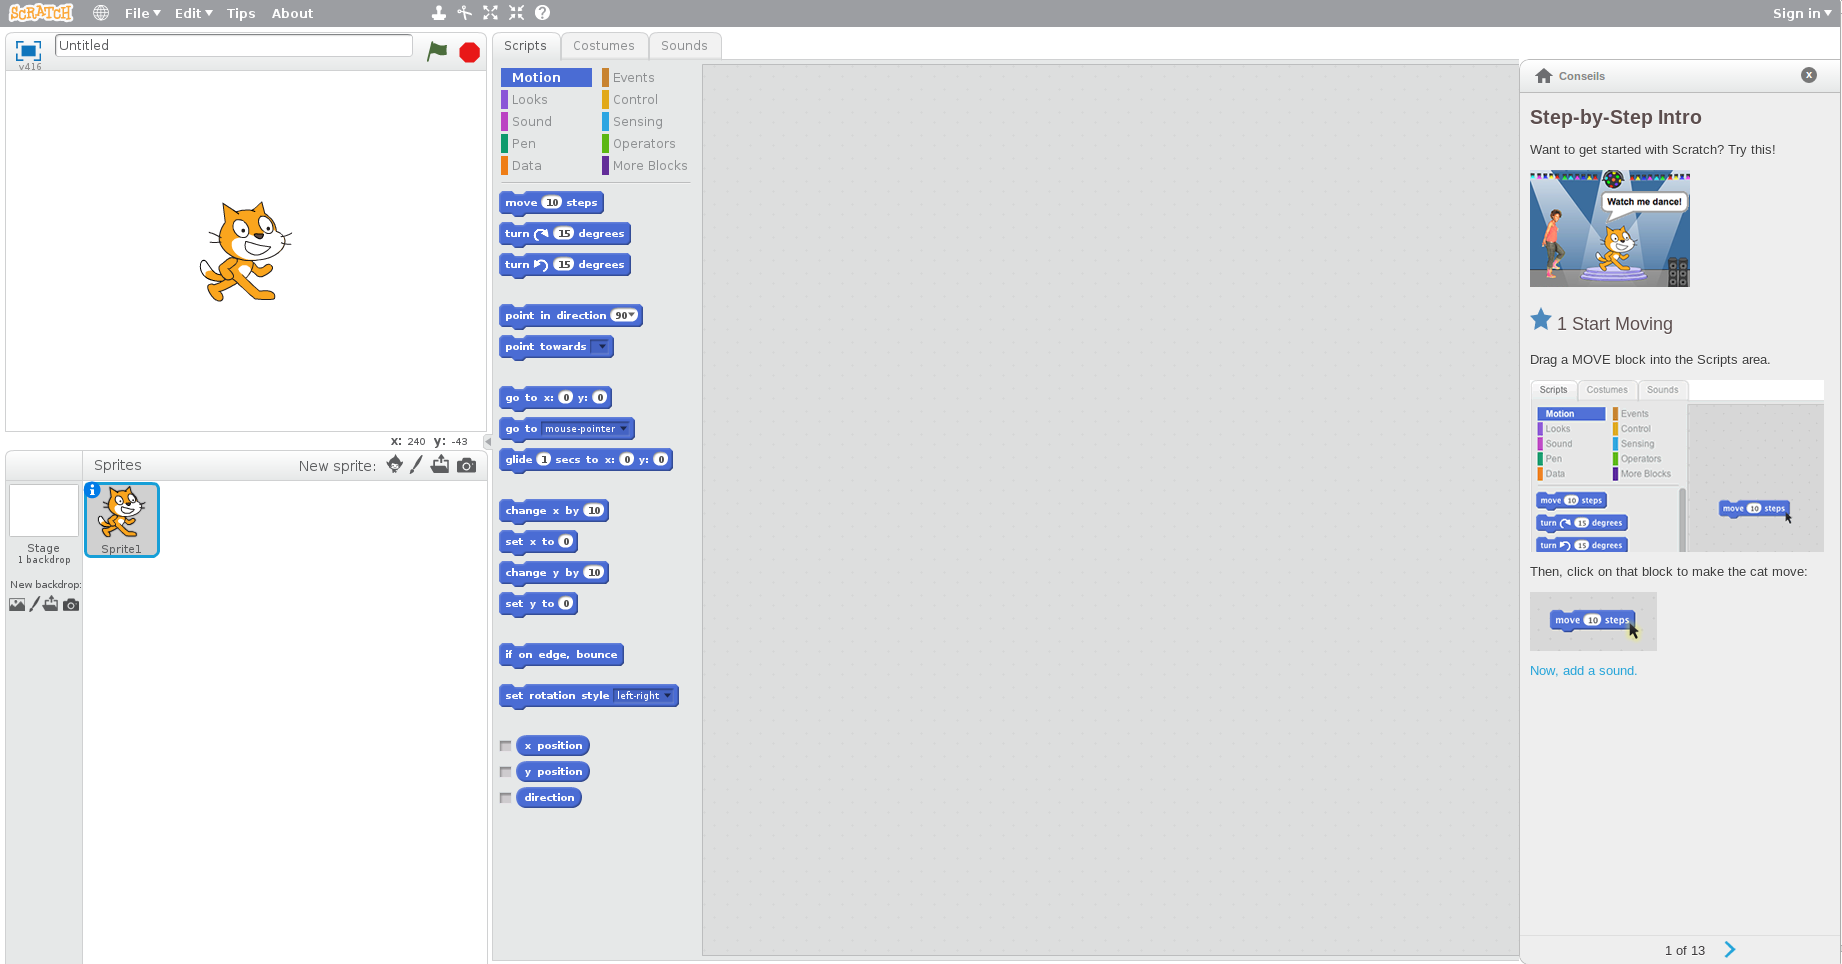
\includegraphics[width=\textwidth]{content/5-related_work/images/scratch-printscreen}
    \caption{Interface de Scratch}
    \label{fig:scratch-printscreen}
  \end{center}
\end{figure}

\subsection{Snap!}

\begin{figure}[!ht]
  \begin{center}
    
\includegraphics[scale=0.07]{content/5-related_work/images/snap}
    \caption{Logo de Snap!}
    \label{fig:snap}
  \end{center}
\end{figure}

Snap! \cite{snap} est un langage de programmation de "glissé-déposé" de \glspl{bloc}. C'est une ré-implémentation et une extension du langage Scratch du MIT. Il a été pensé et conçu pour être orienté web. Il est donc implémenté en JavaScript.\\

Ce langage est né en 2011 et a été créé par Jens Mönig, docteur de l'université de Berkeley. Il se distingue de son père Scratch par l'ajout :
\begin{enumerate}
\item fonctions et procédures de première classe. Une entité dite de première classe est une entité qui supporte toutes les opération disponible sur d'autres entités ; %TODO glossaire premiere classe
\item listes de première classe ;
\item sprite de première classe.
\end{enumerate}

\subsection{Python}

\begin{figure}[!ht]
  \begin{center}
    
\includegraphics[scale=0.4]{content/5-related_work/images/python}
    \caption{Logo de Python}
    \label{fig:python}
  \end{center}
\end{figure}

Python \cite{python} est un langage de programmation qu'il ne faut plus présenter. Il a beaucoup d'avantages dont celui d'avoir une syntaxe légère et d'être facile à prendre en main. Une grande communauté et beaucoup de bibliothèques, dont la fameuse \texttt{turtle}, en fait un excellent langage pour démarrer dans la programmation.

Cependant, devoir apprendre un langage de programmation et la logique informatique en même temps complique la tâche. De plus, lorsqu'on commence un nouveau langage de programmation il faut également apprendre ses bonnes pratiques de codage. %TODO retravailler pour etre neutre

C'est donc un langage qui ne convient pas aux trop jeunes ni à ceux qui ne sont pas vraiment investis dans l'apprentissage de la programmation.

\section{Concepts différenciateurs}
\label{concepts}
Ce chapitre va mettre en lumière les différences et similitudes des méthodes d'apprentissage de la programmation en utilisant à une série de critères tels que le public cible, les moyens, le lieu et les personnes.
\subsection{Pour qui ?}
L'apprentissage de la programmation aux enfants est différenciée sur base de plusieurs critères tels que l'âge, l'origine, la classe sociale, le genre, etc. Les organisations auront donc soit un public visé restreint soit différents programmes pour les groupes d'enfants.

\subsubsection{Âge}
La méthode d'apprentissages doit être différente suivant l'âge. Les enfants n'ont pas tous la maturité pour apprendre des concepts abstraits (boucle, parallélisation...). Par exemple, pour des élèves de maternel, un tableau interactif sera un grand plus car ils n'ont pas encore la dextérité souhaitée pour manipuler la souris. Et au contraire, des enfants plus grands seront plus autonomes et pourront travailler par binôme voir seuls.

\subsubsection{Genre et origine}
Certaines organisations, telle Code.org, mettent l'accent sur la accessibilité pour tous en incitant à la participation des filles qui sont sous-représentées en informatique.

Les personnes qui ne peuvent acquérir un ordinateur ou se payer un stage ne doivent pas être délaissées.

\subsection{Comment ?}
Les principales différences entre toutes les organisations se situent dans la manière d'aborder l'apprentissage. Elles peuvent être de plusieurs ordres, tels que : les outils utilisés, les concepts abordés et l'environnement de travail.

\subsubsection{Outils}
Un aspect pratique qui différencie les apprentissages est le type de langage utilisé. Ici encore différentes écoles s'affrontent.

\paragraph{Le langage réel} Avec ce type de langage, les enfant apprennent la programmation et le langage utilisé. Ces langages sont plus difficiles à prendre en mains mais permette plus d'applications concrètes.
\paragraph{Le langage visuel} Dans la programmation, le plus important est la logique. Un langage qui se rapproche des diagramme allège la syntaxe, par exemple avec un langage de programmation par \glspl{bloc}.
\paragraph{Le langage web} Dans le monde d'aujourd'hui, le web est partout. L'accent doit donc être porté sur l'apprentissage de ce que les enfants voient au quotidien.


\subsubsection{Concepts}
Tous les cours se divisent en deux parties : la théorie et la pratique. Il existe de multiples manières d'assembler les deux dans un cours unique. L'ordre dans lequel les concepts de programmation sont abordés peut se différencier sur plusieurs points:
\begin{itemize}
  \item certains cours commencent par la théorie et demandent ensuite de l'appliquer ;
  \item d'autres proposent des exercices avant d'expliquer ce que les enfants ont utilisé de manière intuitive ;
  \item d'autres encore découpent la matière en petits sous-ensembles avant d'appliquer la première ou la seconde technique.\\
\end{itemize}


Ces différentes façons d'aborder l'apprentissage mènent diverses conceptions de \glspl{mission}. Celles-ci peuvent être très denses ou au contraire une succession de \glspl{mission} simples. Les \glspl{mission} denses sont souvent constituées de nombreux concepts de programmation (boucle, condition, fonction...) pour avoir directement un objectif concret alors que les \glspl{mission} simples essayent de bien séparer l'apprentissage pour fournir une étude la plus progressive possible.\\

Dans certains pays, la programmation est associée aux cours de sciences. Elle devient alors un outil qui perd du même coup une partie de son côté ludique. Par contre, elle touche un plus grand nombre d'enfants.\\

\subsubsection{Environement de travail}
\label{paire}
Les leçons peuvent être organisées de différentes manières :
\begin{description}
  \item[En groupe] L'apprentissage en groupe est souvent réalisé avec un tableau interactif ou un projecteur \footnote{\url{http://scratched.media.mit.edu/resources/scratch-\%C3\%A0-la-maternelle}} ;
  \item[Par binôme] La programmation en binôme est la plus répandue. Faire travailler les enfants par deux les oblige à interagir entre eux et à essayer de résoudre eux-mêmes les problèmes qu'ils rencontrent. Cela permet aussi de diminuer le nombre d'ordinateurs utilisés ;
  \item[Individuel] Cette technique est très peu utilisé, car elle demande beaucoup de moyens matériels et personnels. De plus, lors d'un apprentissage individuel, les étudiants se retrouve vite coincé et demande de l'aide ;
  \item[A domicile] De nombreuses plateformes proposent des cours en ligne qui peuvent être suivis au rythme de chacun. Néanmoins, pour avoir de l'aide, il faut se tourner vers une personne compétente ou vers les forums. Ces formations sont souvent plus théoriques et demandent plus de lecture, ce qui empêche les jeunes enfants de les suivre.
\end{description}

\subsection{De qui ?}
Chaque initiative s'organise suivant différents critères tels que l'intégration ou non dans un programme scolaire, les compétences des encadrants et le système de gestion des ressources

\subsubsection{Type d'organisation}
Les cours d'informatique sont soit donnés dans le cadre d'un programme officiel soit en parascolaire.

Dans le premier cas, les étudiants ne viennent pas tous par choix. Ceci peut entraîner entre autres des blocages et des réticences à participer correctement à l'activité.

Pour les cours donnés en parascolaire, des petites structures très locales se partagent le terrain avec de grandes organisations à visées internationales. Le coût des activités et les horaires en sont les problèmes typiques.

\subsubsection{Encadrants}
La plupart des cours sont donnés par des informaticiens ou au minimum des personnes formées à l'informatique. Mais comme le nombre d'informaticiens est réduit, certaines organisations proposent des cours clés-en-main pour des encadrants sans connaissance particulière en programmation. Ces professeurs apprennent en même temps que leurs étudiants et les aident à réfléchir.\\

Le type de rémunération des encadrants est assez diversifiée. Certains reçoivent des primes en fonction de la réussite de leur classe, d'autres sont payés par l'état ou directement par les étudiants, d'autres encore sont bénévoles.

\subsubsection{Gestion des ressources}
Suivant l'organisation, les cours sont plus ou moins figés. Certaines permettent à leur communauté de créer et/ou de modifier des cours tandis que d'autres ont des équipes dédiées à cette tâche.

